\chapter{Sequences and Series - Grade 12}
\label{mp:s}

\section{Introduction}
In this chapter we extend the arithmetic and quadratic sequences studied in earlier grades, to geometric sequences. We also look at series, which is the summing of the terms in a sequence.

\section{Arithmetic Sequences}
The simplest type of numerical sequence is an \textit{arithmetic sequence}. 

\Definition{Arithmetic Sequence}{An \textit{arithmetic} (or \textit{linear}) \textit{sequence} is a sequence of numbers in which each new term is calculated by \textbf{adding} a constant value to the previous term}

For example,
\nequ{1,2,3,4,5,6,\ldots}
is an arithmetic sequence because you add 1 to the current term to get the next term:
\begin{center}
\begin{tabular}{rl}
first term:&1\\
second term:&2=1+1\\
third term:&3=2+1\\
$\vdots$&\\
$n^{\rm{th}}$ term:&$n=(n-1)+1$\\
\end{tabular}
\end{center}

\Activity{Common Difference}{Find the constant value that is added to get the following sequences and write out the next 5 terms.
\begin{enumerate}
\item{$2,6,10,14,18,22, \ldots$}
\item{$-5,-3,-1,1,3,\ldots$}
\item{$1,4,7,10,13,16,\ldots$}
\item{$-1,10,21,32,43,54,\ldots$}
\item{$3,0,-3,-6,-9,-12, \ldots$}
\end{enumerate}}

\subsection{General Equation for the $n^{th}$-term of an Arithmetic Sequence}

More formally, the number we start out with is called \textit{$a_1$} (the first term), and the difference between each successive term is denoted \textit{d}, called the \textit{common difference}.

The general arithmetic sequence looks like:
\begin{eqnarray*}
a_1 &=& a_1 \\
a_2 &=& a_1 + d \\
a_3 &=& a_2 + d = (a_1 + d) + d = a_1 + 2d \\
a_4 &=& a_3 + d = (a_1 + 2d) + d = a_1 + 3d \\
\ldots \\
a_n &=& a_1 + d \cdot (n - 1)
\end{eqnarray*}

Thus, the equation for the $n^{th}$-term will be:
\begin{equation}
\label{eq:mp:s:arithseq:2}
a_n = a_1 + d \cdot (n - 1)
\end{equation}
Given $a_1$ and the common difference, $d$, the entire set of numbers belonging to an arithmetic sequence can be generated.

\Definition{Arithmetic Sequence}{An \textit{arithmetic} (or \textit{linear}) \textit{sequence} is a sequence of numbers in which each new term is calculated by adding a constant value to the previous term:
\begin{eqnarray}
\label{eq:mp:s:arithseq:1}
a_n = a_{n-1} + d
\end{eqnarray}
where
\begin{itemize}
\item $a_n$ represents the new term, the $n^{th}$-term, that is calculated;
\item $a_{n-1}$ represents the previous term, the $(n-1)^{th}$-term;
\item $d$ represents some constant.
\end{itemize}
}

\Tip{Test for Arithmetic Sequences}{A simple test for an arithmetic sequence is to check that the difference between consecutive terms is constant:
\begin{equation}
a_2 - a_1 = a_3 - a_2 = a_n - a_{n-1} = d
\end{equation}
This is quite an important equation, and is the definitive test for an arithmetic sequence. If this condition does not hold, the sequence is not an arithmetic sequence.}


\Extension{Plotting a graph of terms in an arithmetic sequence}{Plotting a graph of the terms of
sequence sometimes helps in determining the type of sequence involved.
For an arithmetic sequence, plotting $a_n$ vs. $n$ results in:

\begin{center}
\begin{pspicture}(-0.4,-0.8)(8,7.6)
%\psgrid[gridcolor=gray]
\psset{yunit=0.75,xunit=0.75}
\psaxes[arrows=<->,dx=10,Dx=1,dy=10,Dy=1](1,0)(10,10)
\psdots(1,1)(2,2)(3,3)(4,4)(5,5)(6,6)(7,7)(8,8)
\psplot[plotstyle=curve,arrows=->]{1}{8.5}{x}
\psline[linestyle=dashed](7,7)(7,4)(4,4)
\uput[l](7.6,5.1){gradient $d$}
\psarc[arrows=->](5.5,5.4){1}{0}{45}
\uput[u](8.5,8.5){$a_n=a_1 + d(n-1)$}
\uput[l](0.25,5){\rotateleft{Term, $a_n$}}
\uput[r](1,1){$y$-intercept, $a_1$}
\multips(1,0)(1,0){10}{\psline(0,-.1)(0,.1)}
\multips(0,1){10}{\psline(0.9,0)(1.1,0)}
\multido{\n=1+1}{9}{\rput(\n,-0.35){\n}}
\multido{\n=1+1}{9}{\rput(0.65,\n){$a_{\n}$}}
\rput(5,-.75){Index, $n$}
\end{pspicture}
%\caption{When the terms of a linear sequence are plotted as a function of the index, a straight
%line is obtained.}
%\label{fig:mp:extra:linear}
\end{center}
%\end{figure}
%Therefore, we can see that for an arithmetic sequence, the plot of $a_n$ vs. $n$ yields a straight
%line. The gradient (or slope) of the graph represents the common difference, $d$, and the
%$y$-intercept (for $n=1$) represents the first term, $a_1$.
%If we are given the arithmetic sequence,
%\begin{eqnarray*}
%4; \: 6; \:8; \: 10; \: 12; \: \ldots
%\end{eqnarray*}
%and plot each of the terms vs. the corresponding index (subscript), we get a graph of a straight
%line.
%%\begin{figure}[!htbp]
%\begin{center}
%\begin{pspicture}(-1,-1)(10,10)
%\psaxes[arrows=<->,dx=10,Dx=1,dy=10,Dy=1](1,0)(10,10)
%\psplot[plotstyle=dots,plotpoints=9]{1}{9}{x 1 sub 1 mul 1 add}
%\psplot[plotstyle=curve,arrows=->]{1}{9.5}{x 1 sub 1 mul 1 add}
%\uput[u](8.5,19){$a_n=4 + 2(n-1)$}
%\uput[l](0.25,5){\rotateleft{Term, $a_n$}}
%\uput[r](1,1){$y$-intercept, $a_1=1$}
%\multips(1,0)(1,0){9}{\psline(0,-.1)(0,.1)}
%\multips(0,1){10}{\psline(0.9,0)(1.1,0)}
%\multido{\n=1+1}{9}{\rput(\n,-0.35){\n}}
%\multido{\n=1+1}{9}{\rput(0.65,\n){$a_{\n}$}}
%\rput(5,-.75){Index, $n$}
%\end{pspicture}
%\caption{A plot of $a_n$ vs. $n$ for arithmetic sequence \{4; 6; 8; 10; 12; \ldots\}.}
%\label{fig:mp:extra:linearexample}
%\end{center}
%\end{figure}
%We can see that the gradient of the graph is 2, which is equal to the common difference, $d$. The
%first term, $a_1$, is obtained from the $y$-intercept (for $n=1$), which is 4.
}

\section{Geometric Sequences}
%\begin{syllabus}
%\item Identify and solve problems involving number patterns, including but not limited to
%arithmetic and geometric sequences and series.
%\end{syllabus}

\Definition{Geometric Sequences}{A geometric sequence is a sequence in which every number in the
sequence is equal to the previous number in the sequence, \textbf{multiplied} by a constant number.}

This means that the \textit{ratio} between consecutive numbers in the geometric sequence is a
constant. We will explain what we mean by ratio after looking at the following example.

\subsection{Example - A Flu Epidemic}
\Extension{What is influenza?}{Influenza (commonly called ``the flu'') is caused by the influenza
virus, which infects the respiratory tract (nose, throat, lungs). It can cause mild to severe
illness that most of us get during winter time. The main way that the influenza virus is spread is
from person to person in respiratory droplets of coughs and sneezes. (This is called ``droplet
spread''.) This can happen when droplets from a cough or sneeze of an infected person are propelled
(generally, up to a metre) through the air and deposited on the mouth or nose of people nearby. It
is good practise to cover your mouth when you cough or sneeze so as not to infect others around you
when you have the flu.} 

Assume that you have the flu virus, and you forgot to cover your mouth when two friends came to
visit while you were sick in bed. They leave, and the next day they also have the flu. Let's assume
that they in turn spread the virus to two of their friends by the same droplet spread the following
day. Assuming this pattern continues and each sick person infects 2 other friends, we can represent
these events in the following manner:
\begin{figure}[htb]
\begin{center}
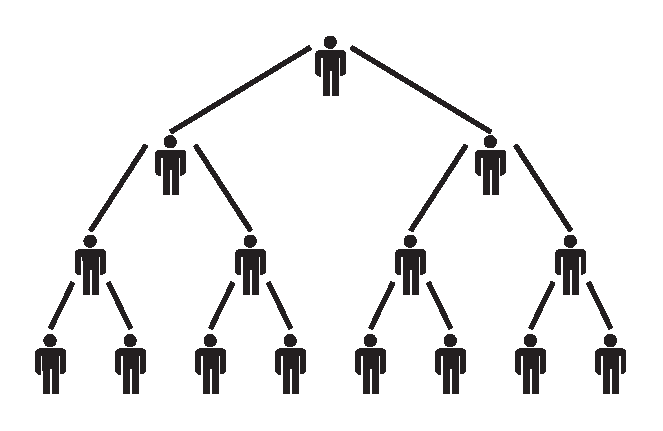
\includegraphics[width=4in]{../ch2sequencesexampleflu.eps}
\caption{Each person infects two more people with the flu virus.}
\label{fig:mp:s:geometricflu}
\end{center}
\end{figure}

Again we can tabulate the events and formulate an equation for the general case:
\begin{center}
\begin{tabular}{|c|l|}\hline
\hline \textbf{Day}, $n$ & \textbf{Number of newly-infected people} \\\hline
\hline 1 & $2 \: \: \: = 2$ \\
\hline 2 & $4 \: \: \: = 2 \times 2 = 2 \times 2^1 $ \\
\hline 3 & $8 \: \: \: = 2 \times 4 = 2 \times 2 \times 2 = 2 \times 2^2$ \\
\hline 4 & $16 \: = 2 \times 8 = 2 \times 2 \times 2 \times 2 = 2 \times 2^3$ \\
\hline 5 & $32 \: = 2 \times 16 = 2 \times 2 \times 2 \times 2 \times 2 = 2 \times 2^4$ \\
\hline \vdots & \qquad \qquad \qquad \qquad \vdots \\
\hline $n$ & $\: \: \quad = 2 \times 2 \times 2 \times 2 \times \ldots \times 2 = 2 \times 2^{n-1}$
\\
\hline\hline
\end{tabular}
\end{center}

The above table represents the number of \textbf{newly-infected} people after $n$ days since you
first infected your 2 friends. 

You sneeze and the virus is carried over to 2 people who start the chain ($a_1 = 2$).
The next day, each one then infects 2 of their friends. Now 4 people are newly-infected.
Each of them infects 2 people the third day, and 8 people are infected, and so on.
These events can be written as a geometric sequence:
\begin{eqnarray*}
2; \: 4; \: 8; \: 16; \: 32; \: \ldots
\end{eqnarray*}

Note the common factor (2) between the events. Recall from the linear arithmetic sequence how the
common difference between terms were established. In the geometric sequence we can determine the
\textit{common ratio}, $r$, by

\begin{equation}
\frac{a_2}{a_1} = \frac{a_3}{a_2} = r
\end{equation}

Or, more general,
\begin{equation}
\label{eq:mp:s:geomseq:1}
\frac{a_n}{a_{n-1}} = r
\end{equation}

\Activity{Common Factor of Geometric Sequence}{Determine the common factor for the following
geometric sequences:
\begin{enumerate}
\item{$5, 10, 20, 40, 80, \ldots$}
\item{$\frac{1}{2},\frac{1}{4},\frac{1}{8},\ldots$}
\item{$7, 28, 112, 448,\ldots$}
\item{$2, 6, 18, 54,\ldots$}
\item{$-3, 30, -300, 3000,\ldots$}
\end{enumerate}}
% -----------------------------------------------------------------

\subsection{General Equation for the $n^{th}$-term of a Geometric Sequence}

From the above example we know $a_1 = 2$ and $r = 2$, and we have seen from the table that the
$n^{th}$-term is given by $a_n = 2 \times 2^{n-1}$. Thus, in general,
\begin{equation}
a_n = a_1 \cdot r^{n-1}
\end{equation}
where $a_1$ is the first term and $r$ is called the \textit{common ratio}. 

So, if we want to know how many people are newly-infected after 10 days, we need to work
out $a_{10}$:
\begin{eqnarray*}
a_n &=& a_1 \cdot r^{n-1} \\
a_{10} &=& 2 \times 2^{10-1} \\
&=& 2 \times 2^9 \\
&=& 2 \times 512 \\
&=& 1024
\end{eqnarray*}

That is, after 10 days, there are 1~024 newly-infected people.

Or, how many days would pass before 16~384 people become newly infected with the flu virus?
\begin{eqnarray*}
a_n &=& a_1 \cdot r^{n-1} \\
16~384 &=& 2 \times 2^{n-1} \\
16~384 \div 2 &=& 2^{n-1} \\
8~192 &=& 2^{n-1} \\
2^{13} &=& 2^{n-1} \\
13 &=& n - 1 \\
n &=& 14
\end{eqnarray*}

That is, 14 days pass before 16~384 people are newly-infected.

\Activity{General Equation of Geometric Sequence}{Determine the formula for the following geometric
sequences:
\begin{enumerate}
\item{$5, 10, 20, 40, 80, \ldots$}
\item{$\frac{1}{2},\frac{1}{4},\frac{1}{8},\ldots$}
\item{$7, 28, 112, 448,\ldots$}
\item{$2, 6, 18, 54,\ldots$}
\item{$-3, 30, -300, 3000,\ldots$}
\end{enumerate}}

%===========================================================

\subsection{Exercises}
\begin{enumerate}
\item{What is the important characteristic of an arithmetic sequence?}
\item{Write down how you would go about finding the formula for the $n^{\rm{th}}$ term of an
arithmetic sequence?}
\item{A single square is made from 4 matchsticks. Two squares in a row needs 7 matchsticks and 3
squares in a row needs 10 matchsticks. Determine:
\begin{enumerate}
\item the first term
\item the common difference
\item the formula for the general term
\item how many matchsticks are in a row of 25 squares
\end{enumerate}
\begin{center}
\begin{pspicture}(0,0)(8,2)
%\psgrid[gridcolor=gray]
\def\match{\psline(0,0)(2,0)\psellipse*(1.8,0)(0.2,0.1)}
\rput(0,0){\match}
\rput{90}(2,0){\match}
\rput{180}(2,2){\match}
\rput{270}(0,2){\match}
\rput(2,0){\rput(0,0){\match}
\rput{90}(2,0){\match}
\rput{180}(2,2){\match}}
\rput(4,0){\rput(0,0){\match}
\rput{90}(2,0){\match}
\rput{180}(2,2){\match}}
\rput(6,0){\rput(0,0){\match}
\rput{90}(2,0){\match}
\rput{180}(2,2){\match}}
\end{pspicture}
\end{center}}
\item{$5;\;x;\;y$ is an arithmetic sequence and $x;\;y\;81$ is a geometric sequence. All terms in
the sequences are integers. Calculate the values of $x$ and $y$.}

\end{enumerate}

\section{Recursive Formulae for Sequences}
%\begin{syllabus}
%\item Correctly interpret recursive formulae: (e.g. $T_{n+1}=T_n+T_{n-1}$).
%\end{syllabus}

When discussing arithmetic and quadratic sequences, we noticed that the difference between two
consecutive terms in the sequence could be written in a general way. 

For an arithmetic sequence, where a new term is calculated by taking the previous term and adding a
constant value, $d$:
\begin{eqnarray*}
a_n = a_{n-1} + d
\end{eqnarray*}
The above equation is an example of a \textit{recursive equation} since we can calculate the
$n^{th}$-term only by considering the previous term in the sequence. Compare this with equation
(\ref{eq:mp:s:arithseq:2}),
\begin{equation}
a_n = a_1 + d \cdot (n - 1)
\end{equation}
where one can directly calculate the $n^{th}$-term of an arithmetic sequence without knowing
previous terms. 

For quadratic sequences, we noticed the difference between consecutive terms is given by
(\ref{eq:mp:s:quadseq:2}):
\begin{eqnarray*}
a_n - a_{n-1} = D \cdot (n-2) + d
\end{eqnarray*}

Therefore, we re-write the equation as
\begin{equation}
a_n = a_{n-1} + D \cdot (n-2) + d
\end{equation}
which is then a recursive equation for a quadratic sequence with common second difference, $D$. 

Using (\ref{eq:mp:s:geomseq:1}), the recursive equation for a geometric sequence is:
\begin{equation}
a_n = r \cdot a_{n-1}
\end{equation}
\\
Recursive equations are extremely powerful: you can work out every term in the series just by
knowing previous terms. As you can see from the examples above, working out $a_n$ using the previous
term $a_{n-1}$ can be a much simpler computation than working out $a_n$ from scratch using a general
formula. This means that using a recursive formula when using a computer to work out a sequence
would mean the computer would finish its calculations significantly quicker.

\Activity{Recursive Formula}{Write the first 5 terms of the following sequences, given their
recursive formulae:
\begin{enumerate}
\item{$a_n=2a_{n-1}+3, a_1=1$}
\item{$a_n=a_{n-1}, a_1=11$}
\item{$a_n=2a^2_{n-1}, a_1=2$}
\end{enumerate}}

\Extension{\textbf{The Fibonacci Sequence}\\
Consider the following sequence:
\begin{eqnarray}
0; \: 1; \: 1; \: 2; \: 3; \: 5; \: 8; \: 13; \: 21; \: 34; \: \ldots
\end{eqnarray}
\\
The above sequence is called the \textit{Fibonacci sequence}. Each new term is calculated by adding the previous two terms. Hence, we can write down the recursive equation:
\begin{eqnarray}
a_n = a_{n-1} + a_{n-2}
\end{eqnarray}}

\section{Series}
\label{mp:se}
In this section we simply work on the concept of \textit{adding} up the numbers belonging to arithmetic and geometric sequences. We call the sum of \textit{any} sequence of numbers a \textit{series}.

\subsection{Some Basics}
If we add up the terms of a sequence, we obtain what is called a \textit{series}. If we only sum a finite amount of terms, we get a \textit{finite series}. We use the symbol $S_n$ to mean the sum of the first $n$ terms of a sequence
$\{a_1; \: a_2; \: a_3; \ldots ; a_n \}$:
\begin{eqnarray}
S_n = a_1 + a_2 + a_3 + \ldots + a_n
\end{eqnarray}

For example, if we have the following sequence of numbers
\begin{eqnarray*}
1; \: 4; \: 9; \: 25; \: 36; \: 49; \: \ldots
\end{eqnarray*}
and we wish to find the sum of the first 4 terms, then we write
\begin{eqnarray*}
S_4 = 1 + 4 + 9 + 25 = 39
\end{eqnarray*}
The above is an example of a finite series since we are only summing 4 terms.

If we sum infinitely many terms of a sequence, we get an \textit{infinite series}:
\begin{eqnarray}
S_\infty = a_1 + a_2 + a_3 + \ldots
\end{eqnarray}

\subsection{Sigma Notation}
%\begin{syllabus}
%\item Correctly interpret sigma notation.
%\end{syllabus}

In this section we introduce a notation that will make our lives a little easier.

A sum may be written out using the summation symbol $\sum$\,. This symbol is \textit{sigma}, which is the capital letter ``S'' in the Greek alphabet. It indicates that you must sum the expression to the \textit{right} of it:
\begin{equation}
\label{eq:mp:se:sigma}
\sum_{i=m}^n a_i = a_m + a_{m+1} + \ldots + a_{n-1}+ a_n
\end{equation}
where
\begin{itemize}
\item $i$ is the index of the sum;
\item $m$ is the lower bound (or start index), shown below the summation symbol;
\item $n$ is the upper bound (or end index), shown above the summation symbol;
\item $a_i$ are the terms of a sequence.
\end{itemize}

The index $i$ is increased from $m$ to $n$ in steps of $1$.

If we are summing from $n=1$ (which implies summing from the first term in a sequence), then we can use either $S_n$- or $\sum$-notation since they mean the same thing:
\begin{equation}
\label{eq:mp:se:Ssigma}
S_n=\sum_{i=1}^n a_i = a_1 + a_2 + \ldots + a_n
\end{equation}

For example, in the following sum,
\begin{equation*}
\sum_{i=1}^5 i
\end{equation*}
we have to add together all the terms in the sequence $a_i=i$ from $i=1$ up until $i=5$:
\begin{equation*}
\sum_{i=1}^5 i = 1 + 2 + 3 + 4 + 5 = 15
\end{equation*}

\subsubsection{Examples}

\begin{enumerate}
\item
\begin{eqnarray*}
\sum_{i=1}^6 2^i &=& 2^1 + 2^2 + 2^3 + 2^4 + 2^5 + 2^6 \\
&=& 2 + 4 + 8 + 16 + 32 + 64 \\
&=& 126
\end{eqnarray*}
\item
\begin{eqnarray*}
\sum_{i=3}^{10} (3x^i) = 3x^3 + 3x^4 + \ldots + 3x^9 + 3x^{10}
\end{eqnarray*}
for any value $x$.
\end{enumerate}

\subsubsection{Some Basic Rules for Sigma Notation}

\begin{enumerate}
\item {Given two sequences, $a_i$ and $b_i$,
\begin{eqnarray}
\label{eq:mp:series:sigma:rule1}
\sum_{i=1}^n (a_i + b_i) &=& \sum_{i=1}^n a_i + \sum_{i=1}^n b_i
\end{eqnarray}
}

\item {For any constant $c$ that is not dependent on the index $i$,
\begin{eqnarray}
\label{eq:mp:series:sigma:rule2}
\sum_{i=1}^n c \cdot a_i &=& c \cdot a_1 + c \cdot a_2 + c \cdot a_3 + \ldots + c \cdot a_n \nonumber \\
&=& c \; (a_1 + a_2 + a_3 + \ldots + a_n) \nonumber \\
&=& c \sum_{i=1}^n a_i
\end{eqnarray}
}
\end{enumerate}

\subsubsection{Exercises}
\begin{enumerate}
\item What is $\sum_{k=1}^4 \limits 2$?
\item Determine $\sum_{i=-1}^3 \limits i$.
\item Expand $\sum_{k=0}^5 \limits i$.
\item{Calculate the value of $a$ if:
\nequ{\sum_{k=1}^{3}a\cdot 2^{k-1}=28}}
\end{enumerate}

%\begin{syllabus}
%\item Grade 12
%\item Prove and correctly select the formula for and calculate the sum of series, including:
%\begin{eqnarray*}
%\sum_{i=1}^n 1 &=& n \\
%\sum_{i=1}^n i^2 &=& \frac{n(2n+1)(n+1)}{6} \mbox{ not in syllabus, mark as extra}\\
%\sum_{i=1}^n i &=& \frac{n(n+1)}{2} \\
%\sum_{i=1}^n a+(i-1)d &=& \frac n2 (2a+(n-1))\\
%\sum_{i=1}^n a.r^{i-1} &=& \frac{a(r^n-1)}{r-1}\\
%\sum_{i=1}^\infty a.r^{i-1} &=& \frac a{1-r} \qquad -1<1
%\end{eqnarray*}
%\end{syllabus}

\section{Finite Arithmetic Series}

Remember that an arithmetic sequence is a set of numbers, such that the difference between any term and the previous term is a constant number, $d$, called the \textbf{constant difference}:
\begin{eqnarray}
\label{eq:mp:series:lin:gen}
a_n = a_1 + d \; (n - 1)
\end{eqnarray}
where
\begin{itemize}
\item $n$ is the index of the sequence;
\item $a_n$ is the $n^{th}$-term of the sequence;
\item $a_1$ is the first term;
\item $d$ is the common difference.
\end{itemize}

When we sum a finite number of terms in an arithmetic sequence, we get a \textit{finite arithmetic series}.

The simplest arithmetic sequence is when $a_1=1$ and $d=0$ in the general form \eqref{eq:mp:series:lin:gen}; in other words all the terms in the sequence are 1:
\begin{eqnarray*}
a_i &=& a_1 + d \; (i - 1) \\
&=& 1 + 0 \cdot (i - 1) \\
&=& 1 \\
\{a_i\} &=& \{1; \: 1; \: 1; \: 1; \: 1; \: \ldots \}
\end{eqnarray*}
If we wish to sum this sequence from $i=1$ to any positive integer $n$, we would write
\begin{equation*}
\sum_{i=1}^n {a_i} = \sum_{i=1}^n 1 = 1 + 1 + 1 + \ldots + 1 \qquad (n\textrm{ times})
\end{equation*}

Since all the terms are equal to 1, it means that if we sum to $n$ we will be adding $n$-number of $1$'s together, which is simply equal to $n$:
\begin{equation}
\boxed{\sum_{i=1}^n 1 = n}
\end{equation}

Another simple arithmetic sequence is when $a_1=1$ and $d=1$, which is the sequence of positive integers:
\begin{eqnarray*}
a_i &=& a_1 + d \; (i - 1) \\
&=& 1 + 1 \cdot (i - 1) \\
&=& i \\
\{a_i\} &=& \{1; \: 2; \: 3; \: 4; \: 5; \: \ldots \}
\end{eqnarray*}
If we wish to sum this sequence from $i=1$ to any positive integer $n$, we would write
\begin{equation}
\label{eq:mp:se:fa:simple:sum1}
\sum_{i=1}^n i = 1 + 2 + 3 + \ldots + n
\end{equation}
This is an equation with a very important solution as it gives the answer to the sum of positive integers.

\begin{IFact}{Mathematician, Karl Friedrich Gauss, discovered this proof when he was only 8 years old. His teacher had decided to give his class a problem which would distract them for the entire day by asking them to add all the numbers from 1 to 100. Young Karl realised how to do this almost instantaneously and shocked the teacher with the correct answer, 5050.}
\end{IFact}

We first write $S_n$ as a sum of terms in ascending order:
\begin{equation}
\label{eq:mp:series:arith:sum_integers1}
S_n = 1 + 2 + \ldots + (n - 1) + n
\end{equation}
\noindent
We then write the same sum but with the terms in descending order:
\begin{equation}
\label{eq:mp:series:arith:sum_integers2}
S_n = n + (n-1) + \ldots + 2 + 1
\end{equation}
We then add corresponding pairs of terms from equations \eqref{eq:mp:series:arith:sum_integers1} and \eqref{eq:mp:series:arith:sum_integers2}, and we find that the sum for each pair is the same, $(n+1)$:
\begin{equation}
2 \; S_n = (n+1) + (n+1) + \ldots + (n+1) + (n+1)
\end{equation}
We then have $n$-number of $(n+1)$-terms, and by simplifying we arrive at the final result:
\begin{eqnarray*}
2 \; S_n &=& n \; (n + 1) \\
S_n &=& \frac {n}{2} \; (n + 1)
\end{eqnarray*}
\begin{equation}
\label{eq:mp:series:sum_integers}
\boxed{S_n = \sum_{i=1}^n i = \frac {n}{2} \; (n + 1)}
\end{equation}
Note that this is an example of a quadratic sequence.

\subsection{General Formula for a Finite Arithmetic Series}
If we wish to sum any arithmetic sequence, there is no need to work it out term-for-term. We will now determine the general formula to evaluate a finite arithmetic series. We start with the general formula for an arithmetic sequence and sum it from $i=1$ to any positive integer $n$:
\begin{eqnarray*}
\sum_{i=1}^n a_i &=& \sum_{i=1}^n \; [a_1 + d \, (i-1)] \\
&=& \sum_{i=1}^n \; (a_1 + di - d) \\
&=& \sum_{i=1}^n \; [(a_1 - d) + di] \\
&=& \sum_{i=1}^n \; (a_1 - d) + \sum_{i=1}^n \; (di) \\
&=& \sum_{i=1}^n \; (a_1 - d) + d \; \sum_{i=1}^n \; i \\
&=& (a_1 - d) \, n + \frac {dn}{2} \; (n + 1) \\
&=& \frac{n}{2} \: (2a_1 - 2d + dn + d) \\
&=& \frac{n}{2} \: (2a_1 + dn - d) \\
&=& \frac{n}{2} \: [\, 2a_1 + d \, (n - 1) \,]
\end{eqnarray*}
So, the general formula for determining an arithmetic series is given by
\begin{equation}
\label{eq:mp:se:fa:3}
\boxed {S_n = \sum_{i=1}^n \; [\, a_1 + d \, (i-1) \,] = \frac{n}{2} \: [\, 2a_1 + d \, (n - 1) \,]}
\end{equation}
For example, if we wish to know the series $S_{20}$ for the arithmetic sequence $a_i= 3 + 7 \, (i-1)$, we could either calculate each term individually and sum them:
\begin{eqnarray*}
S_{20} &=& \sum_{i=1}^{20} \; [3 + 7 \, (i-1)] \\
&=& 3 + 10 + 17 + 24 + 31 + 38 + 45 + 52 + \\
&& 59 + 66 + 73 + 80 + 87 + 94 + 101 + \\
&& 108 + 115 + 122 + 129 + 136 \\
&=& 1390
\end{eqnarray*}
or, more sensibly, we could use equation \eqref{eq:mp:se:fa:3} noting that $a_1=3$, $d=7$ and $n=20$ so that
\begin{eqnarray*}
\label{eq:mp:se:fa:ex:smartway}
S_{20} &=& \sum_{i=1}^{20} \; [3 + 7 \, (i-1)] \\
&=& \textstyle \small {\frac{20}{2}} \: [2 \cdot 3 + 7 \, (20 - 1) ] \\
&=& 1390
\end{eqnarray*}
This example demonstrates how useful equation \eqref{eq:mp:se:fa:3} is.

\subsection{Exercises}
\begin{enumerate}

\item The sum to $n$ terms of an arithmetic series is $S_n = \dfrac{n}{2} \, (7n + 15)$.
\begin{enumerate}
\item{How many terms of the series must be added to give a sum of 425?}
\item{Determine the 6$^{th}$ term of the series.}
\end{enumerate}

\item The sum of an arithmetic series is $100$ times its first term, while the last term is $9$ times the first term. Calculate the number of terms in the series if the first term is not equal to zero.

\item The common difference of an arithmetic series is $3$. Calculate the values of $n$ for which the $n^{th}$ term of the series is $93$, and the sum of the first $n$ terms is 975.

\item The sum of $n$ terms of an arithmetic series is $5n^2 - 11n$ for all values of $n$. Determine the common difference.

\item{The sum of an arithmetic series is 100 times the value of its first term, while the last term is 9 times the first term. Calculate the number of terms in the series if the first term is not equal to zero.}

\item{The third term of an arithmetic sequence is -7 and the 7$^{th}$ term is 9. Determine the sum of the first 51 terms of the sequence.}

\item{Calculate the sum of the arithmetic series $4+7+10+\cdots+901$.}
\item{ The common difference of an arithmetic series is 3. Calculate the values of $n$ for which the $n^{\rm{th}}$ term of the series is 93 and the sum of the first $n$ terms is 975.}
\end{enumerate}

\section{Finite Squared Series}
When we sum a finite number of terms in a quadratic sequence, we get a \textit{finite
quadratic series}. The general form of a quadratic series is quite complicated,
so we will only look at the simple case when $D=2$ and $d=(a_2 - a_1)=3$, where $D$ is the common second difference and $d$ is the finite difference. This is the sequence of squares of the integers:
\begin{eqnarray*}
\label{eq:mp:se:quad:seq}
a_i &=& i^{\,2} \\
\{a_i\} &=& \{1^2; \: 2^2; \: 3^2; \: 4^2; \: 5^2; \: 6^2; \: \ldots \} \\
&=& \{1; \: 4; \: 9; \: 16; \: 25; \: 36; \: \ldots \}
\end{eqnarray*}
If we wish to sum this sequence and create a series, then we write
\begin{equation*}
\label{eq:mp:se:fs:sum}
S_n=\sum_{i=1}^n i^{\,2} = 1 + 4 + 9 + \ldots + n^2
\end{equation*}
which can be written, in general, as
\begin{equation}
\label{eq:mp:se:fs:2}
\boxed{S_n = \sum_{i=1}^n i^2 = \frac{n}{6}(2n + 1)(n + 1)}
\end{equation}
\\
The proof for equation \eqref{eq:mp:se:fs:2} can be found under the Advanced block that follows:
\\
\Extension{Derivation of the Finite Squared Series}{
We will now prove the formula for the finite squared series:
\begin{equation*}
S_n=\sum_{i=1}^n i^{\,2} = 1 + 4 + 9 + \ldots + n^2
\end{equation*}
We start off with the expansion of ${(k + 1)}^3$.
\begin{eqnarray*}
{(k + 1)}^3 &=& k^3 + 3k^2 + 3k + 1 \\
{(k + 1)}^3 - k^3 &=& 3k^2 + 3k + 1
\end{eqnarray*}
\begin{eqnarray*}
k=1 &:& \quad 2^3 - 1^3 = 3(1)^2 + 3(1) + 1 \\
\vspace{6pt} \\
k=2 &:& \quad 3^3 - 2^3 = 3(2)^2 + 3(2) + 1 \\
\vspace{6pt} \\
k=3 &:& \quad 4^3 - 3^3 = 3(3)^2 + 3(3) + 1 \\
&\vdots& \\
k=n &:& \quad {(n + 1)}^3 - n^3 = 3n^2 + 3n + 1
\end{eqnarray*}
If we add all the terms on the right and left, we arrive at
\begin{eqnarray*}
{(n + 1)}^3 - 1 &=& \sum_{i=1}^n \: (3i^2 + 3i + 1) \\
\vspace{12pt} \\
n^3 + 3n^2 + 3n + 1 - 1 &=& 3\,\sum_{i=1}^n \: i^2 + 3\,\sum_{i=1}^n \: i + \sum_{i=1}^n \: 1 \\
\vspace{12pt} \\
n^3 + 3n^2 + 3n &=& 3\,\sum_{i=1}^n \: i^2 + \frac{3n}{2}\,(n + 1) + n \\
\vspace{12pt} \\
\sum_{i=1}^n \: i^2 &=& \frac{1}{3}\,[n^3 + 3n^2 + 3n - \frac{3n}{2}\,(n + 1) - n] \\
\vspace{12pt} \\
&=& \frac{1}{3}\,(n^3 + 3n^2 + 3n - \frac{3}{2}\,n^2 - \frac{3}{2}\,n - n) \\
\vspace{12pt} \\
&=& \frac{1}{3}\,(n^3 + \frac{3}{2}\,n^2 + \frac{1}{2}\,n) \\
\vspace{12pt} \\
&=& \frac{n}{6}\,(2n^2 + 3n + 1)
\end{eqnarray*}
Therefore,
\begin{equation*}
\boxed{\sum_{i=1}^n \: i^2 = \frac{n}{6}(2n + 1)(n + 1)}
\end{equation*}}


\section{Finite Geometric Series}
When we sum a known number of terms in a geometric sequence, we get a \textit{finite geometric series}. %We know from \eqref{eq:mp:s:geom:genalt}, that 
We can write out each term of a geometric sequence in the general form:
\begin{equation}
a_n = a_1 \cdot r^{n-1}
\end{equation}
where
\begin{itemize}
\item $n$ is the index of the sequence;
\item $a_n$ is the $n^{th}$-term of the sequence;
\item $a_1$ is the first term;
\item $r$ is the common ratio (the ratio of any term to the previous term).
\end{itemize}

\vspace{12pt}
By simply adding together the first $n$ terms, we are actually writing out the series
\begin{equation}
\label{eq:mp:s:geom:S}
S_n = a_1 + a_1\,r + a_1\,r^2 + \ldots + a_1\,r^{n-2} + a_1\,r^{n-1}
\end{equation}
We may multiply the above equation by $r$ on both sides, giving us
\begin{equation}
\label{eq:mp:s:geom:rS}
rS_n = a_1\,r + a_1\,r^2 + a_1\,r^3 + \ldots + a_1\,r^{n-1} + a_1\,r^n
\end{equation}
You may notice that all the terms on the right side of \eqref{eq:mp:s:geom:S} and \eqref{eq:mp:s:geom:rS} are the same, except the first and last terms. If we subtract \eqref{eq:mp:s:geom:S} from \eqref{eq:mp:s:geom:rS}, we are left with just
\begin{eqnarray*}
\label{eq:mp:s:geom:proof}
rS_n - S_n = a_1\,r^n - a_1 \\
S_n(r - 1) = a_1\,(r^n - 1)
\end{eqnarray*}
Dividing by $(r-1)$ on both sides, we arrive at the general form of a geometric series:
\begin{equation}
\label{eq:mp:se:fg:4}
\boxed{S_n = \sum_{i=1}^n a_1 \cdot r^{i-1} = \frac{a_1 \, (r^n - 1)}{r-1}}
\end{equation}
The following video summarises what you have learnt so far about sequences and series:
Khan Academy video on sequences and series, part 1:SIYAVULA-VIDEO:http://cnx.org/content/m39301/latest/#series-1
\subsection{Exercises}
\begin{enumerate}
\item Prove that $$a + ar + ar^2 + ... + ar^{n-1} = \dfrac{a\,(1 - r^n)}{(1-r)}$$
\item Find the sum of the first 11 terms of the geometric series $6 + 3 + \tfrac{3}{2} + \tfrac{3}{4} + \ldots$
\item Show that the sum of the first $n$ terms of the geometric series $$54 + 18 + 6 + ... + 5 \, (\tfrac{1}{3})^{n-1}$$ is given by $81 - 3^{4-n}$.
\item The eighth term of a geometric sequence is $640$. The third term is $20$. Find the sum of the first 7 terms.
\item Solve for $n$: $\sum_{t=1}^n \limits 8 \, (\tfrac{1}{2})^t = 15\tfrac{3}{4}$.
\item The ratio between the sum of the first three terms of a geometric series and the sum of the $4^{th}$-, $5^{th}$- and $6^{th}$-terms of the same series is $8:27$. Determine the common ratio and the first 2 terms if the third term is $8$.
\item{Given the geometric sequence $1;\;-3;\; 9;\;\dots$ determine:
\begin{enumerate}
\item{The 8$^{\rm{th}}$ term of the sequence}
\item{The sum of the first 8 terms of the sequence.}
\end{enumerate}}
\item{Determine:
\nequ{\sum_{n=1}^{4}3\cdot2^{n-1}}}
\end{enumerate}

\section{Infinite Series}
Thus far we have been working only with finite sums, meaning that whenever we determined the sum of a series, we only considered the sum of the first $n$ terms. In this section, we consider what happens when we add infinitely many terms together. You might think that this is a silly question - surely the answer will be $\infty$ when one sums infinitely many numbers, no matter how small they are? The surprising answer is that while in some cases one will reach $\infty$ (like when you try to add all the positive integers together), there are some cases one will get a finite answer. If you don't believe this, try doing the following sum, a geometric series, on your calculator or computer:
$$\tfrac{1}{2} + \tfrac{1}{4} + \tfrac{1}{8} + \tfrac{1}{16} + \tfrac{1}{32} + \ldots $$
You might think that if you keep adding more and more terms you will eventually get larger and larger numbers, but in fact you won't even get past $1$ - try it and see for yourself!

We denote the sum of an infinite number of terms of a sequence by
\begin{eqnarray*}
S_\infty = \sum^\infty_{i=1} a_i
\end{eqnarray*}

When we sum the terms of a series, and the answer we get after each summation gets closer and closer to some number, we say that the series \textit{converges}. If a series does not converge, then we say that it \textit{diverges}.

\subsection{Infinite Geometric Series}

There is a simple test for knowing instantly which geometric series converges and which diverges. When $r$, the common ratio, is strictly between -1 and 1, i.e. $-1 < r < 1$, the infinite series will converge, otherwise it will diverge. There is also a formula for working out the value to which the series converges.

Let's start off with formula \eqref{eq:mp:se:fg:4} for the finite geometric series:
\begin{equation*}
S_n = \sum_{i=1}^n a_1 \cdot r^{i-1} = \frac{a_1 \, (r^n - 1)}{r-1}
\end{equation*}

Now we will investigate the behaviour of $r^n$ for $-1<r<1$ as n becomes larger.

Take $r=\frac{1}{2}$:
\begin{eqnarray*}
n=1 &:& r^n = r^1 =(\tfrac{1}{2})^1 = \tfrac{1}{2} \\
n=2 &:& r^n = r^2 =(\tfrac{1}{2})^2 = \tfrac{1}{2} \cdot \tfrac{1}{2} = \tfrac{1}{4} < \tfrac{1}{2} \\
n=3 &:& r^n = r^3 =(\tfrac{1}{2})^3 = \tfrac{1}{2} \cdot \tfrac{1}{2} \cdot \tfrac{1}{2} = \tfrac{1}{8} < \tfrac{1}{4}
\end{eqnarray*}

Since $r$ is in the range $-1<r<1$, we see that $r^n$ gets closer to $0$ as n gets larger.

Therefore,
\begin{eqnarray*}
S_n &=& \frac{a_1 \, (r^n - 1)}{r - 1} \\
\vspace{12pt} \\
S_\infty &=& \frac{a_1 \, (0 - 1)}{r - 1} \qquad \mathrm{ for } -1 < r < 1 \\
\vspace{12pt} \\
&=& \frac {-a_1}{r - 1} \\
\vspace{12pt} \\
&=& \frac {a_1}{1 - r}
\end{eqnarray*}

The sum of an infinite geometric series is given by the formula
\begin{eqnarray}
\label{eq:mp:se:ig:4}
\boxed{S_\infty = \sum_{i=1}^\infty a_1r^{i-1} = \frac {a_1}{1-r} \qquad \mathrm{ for } \qquad -1<r<1 }
\end{eqnarray}
where $a_1$ is the first term of the series and $r$ is the common ratio.
Khan Academy video on sequences and series, part 2:SIYAVULA-VIDEO:http://cnx.org/content/m39301/latest/#series-2

\subsection{Exercises}
\begin{enumerate}
\item What does $(\tfrac{2}{5})^n$ approach as $n$ tends towards $\infty$?
\item{Given the geometric series:
\nequ{2\cdot(5)^5+2\cdot(5)^4+2\cdot(5)^3+\ldots}
\begin{enumerate}
\item Show that the series converges
\item Calculate the sum to infinity of the series
\item Calculate the sum of the first 8 terms of the series, correct to two decimal places.
\item Determine
\nequ{\sum_{n=9}^{\infty}2\cdot{5}^{6-n}}
correct to two decimal places using previously calculated results.
\end{enumerate}}
\item Find the sum to infinity of the geometric series $3 + 1 + \tfrac{1}{3} + \tfrac{1}{9} + \ldots$
\item Determine for which values of $x$, the geometric series $$2 + \tfrac{2}{3} \, (x+1) +\tfrac{2}{9} \, (x+1)^2 + \ldots$$ will converge.
\item The sum to infinity of a geometric series with positive terms is $4\tfrac{1}{6}$ and the sum of the first two terms is $2\tfrac{2}{3}$. Find $a$, the first term, and $r$, the common ratio between consecutive terms.
\end{enumerate}


\section{End of Chapter Exercises}
\begin{enumerate}

\item Is $1 + 2 + 3 + 4 + ...$ an example of a \textit{finite series} or an \textit{infinite series}?

\item Calculate $$\sum_{k=2}^6 3 \, {(\tfrac{1}{3})}^{k+2}$$

\item If $x+1$; $x-1$; $2x-5$ are the first 3 terms of a convergent geometric series, calculate the:
\begin{enumerate}
\item Value of $x$.
\item Sum to infinity of the series.
\end{enumerate}

\item Write the sum of the first 20 terms of the series $6 + 3 + \tfrac{3}{2} + \tfrac{3}{4} + ...$ in $\sum$\,-notation.

\item Given the geometric series: $2 \cdot 5^5 + 2 \cdot 5^4 + 2 \cdot 5^3 + \ldots$
\begin{enumerate}
\item Show that the series converges.
\item Calculate the sum of the first 8 terms of the series, correct to TWO decimal places.
\item \label{Cumulative:1} Calculate the sum to infinity of the series.
\item Use your answer to \ref{Cumulative:1} above to determine $$\sum_{n=9}^\infty 2 \cdot 5^{(6-n)}$$ correct to TWO decimal places.
\end{enumerate}

\item For the geometric series, $$54 + 18 + 6 + ... + 5 \, (\tfrac{1}{3})^{n-1}$$ calculate the smallest value of $n$ for which the sum of the first $n$ terms is greater than $80.99$.

\item Determine the value of $\sum_{k=1}^\infty \limits 12(\tfrac{1}{5})^{k-1} $.

\item A new soccer competition requires each of $8$ teams to play every other team once.
\begin{enumerate}
\item Calculate the total number of matches to be played in the competition.
\item If each of $n$ teams played each other once, determine a formula for the total number of matches in terms of $n$.
\end{enumerate}

\item The midpoints of the opposite sides of square of length $4$ units are joined to form 4 new smaller squares. This midpoints of the new smaller squares are then joined in the same way to make even smaller squares. This process is repeated indefinitely. Calculate the sum of the areas of all the squares so formed.

\item Thembi worked part-time to buy a Mathematics book which cost R29,50. On 1 February she saved R1,60, and saves everyday 30 cents more than she saved the previous day. (So, on the second day, she saved R1,90, and so on.) After how many days did she have enough money to buy the book?

\item Consider the geometric series: $$5 + 2\tfrac{1}{2} + 1\tfrac{1}{4} + \ldots $$
\begin{enumerate}
\item If $A$ is the sum to infinity and $B$ is the sum of the first $n$ terms, write down the value of:
\begin{enumerate}
\item $A$
\item $B$ in terms of $n$.
\end{enumerate}

\item For which values of $n$ is $(A - B) < \tfrac{1}{24}$?
\end{enumerate}

\item A certain plant reaches a height of $118$ mm after one year under ideal conditions in a greenhouse. During the next year, the height increases by $12$ mm. In each successive year, the height increases by $\tfrac{5}{8}$ of the previous year's growth. Show that the plant will never reach a height of more than $150$ mm.

\item Calculate the value of $n$ if $\sum_{a=1}^n \limits \, (20 - 4a) = -20$.

\item Michael saved R400 during the first month of his working life. In each subsequent month, he saved 10\% more than what he had saved in the previous month.
\begin{enumerate}
\item How much did he save in the $7^{th}$ working month?
\item How much did he save all together in his first $12$ working months?
\item In which month of his working life did he save more than R1,500 for the first time?
\end{enumerate}

\item A man was injured in an accident at work. He receives a disability grant of R4,800 in the first year. This grant increases with a fixed amount each year.
\begin{enumerate}
\item What is the annual increase if, over $20$ years, he would have received a total of R143,500?
\item His initial annual expenditure is R2,600 and increases at a rate of R400 per year. After how many years does his expenses exceed his income?
\end{enumerate}
\item{The Cape Town High School wants to build a school hall and is busy with fundraising. Mr. Manuel, an ex-learner of the school and a successful politician, offers to donate money to the school. Having enjoyed mathematics at school, he decides to donate an amount of money on the following basis.
He sets a mathematical quiz with 20 questions. For the correct answer to the first question (any learner may answer), the school will receive 1 cent, for a correct answer to the second question, the school will receive 2 cents, and so on. The donations 1, 2, 4, ... form a geometric sequence. Calculate (Give your answer to the nearest Rand)
\begin{enumerate}
\item{The amount of money that the school will receive for the correct answer to the 20$^{\rm{th}}$ question.}
\item{The total amount of money that the school will receive if all 20 questions are answered correctly.}
\end{enumerate}
}
\item{The first term of a geometric sequence is 9, and the ratio of the sum of the first eight terms to the sum of the first four terms is $97:81$. Find the first three terms of the sequence, if it is given that all the terms are positive.}

\item{$(k-4); \; (k+1); \; m; \; 5k$ is a set of numbers, the first three of which form an arithmetic sequence, and the last three a geometric sequence. Find $k$ and $m$ if both are positive.}

\item{Given: The sequence $6+p \;\!; \; 10+p\;\!; \; 15+p \;$ is geometric.}
\begin{enumerate}
\item{Determine $p$.}
\item{Show that the common ratio is $\tfrac{5}{4}$.}
\item{Determine the $10^{th}$ term of this sequence correct to one decimal place.}
\end{enumerate}

\item{The second and fourth terms of a convergent geometric series are $36$ and $16$, respectively. Find the sum to infinity of this series, if all its terms are positive.}

\item{Evaluate: $\sum_{k=2}^5 \limits \dfrac{k(k+1)}{2}$}

\item{$S_n = 4n^2 + 1$ represents the sum of the first $n$ terms of a particular series. Find the second term.}

\item{Find $p$ if: \qquad $\sum_{k=1}^{\infty} \limits \; 27p^{ k} = \sum_{t=1}^{12} \limits \; (24-3t)$}

\item{Find the integer that is the closest approximation to:$$\dfrac{10^{ 2001} \:+\: 10^{ 2003}}{10^{ 2002} \:+\: 10^{ 2002}}$$}

\item{Find the pattern and hence calculate: $$1-2+3-4+5-6 \ldots +677 - 678 + \ldots -1000$$}

\item{Determine if $\sum_{p=1}^{\infty} \limits (x+2)^p$ converges. If it does, then work out what it converges to if:}
\begin{enumerate}
\item{$x=-\dfrac{5}{2}$}
\item{$x=-5$}
\end{enumerate}

\item{Calculate: \qquad $\sum_{i=1}^{\infty} \limits \; 5 \cdot 4^{-i}$}

\item{The sum of the first $p$ terms of a sequence is $p \; (p+1)$. Find the $10^{th}$ term.}

\item{The powers of $2$ are removed from the set of positive integers $$1; \: 2; \: 3; \: 4; \: 5; \: 6; \ldots; 1998; \: 1999; \: 2000$$ Find the sum of remaining integers.}

\item{Observe the pattern below:

\begin{pspicture}(-3, -6)(6, 6)
%\psgrid[gridlabels=10pt,gridlabelcolor=black]
%\psaxes[labels=none, ticks=all]{<->}(0, 0)(-4.5, -2.5)(5,3.5)
\psline(6, 6)(0, 0)(6, -6)
\uput[0](1, 0){A}
\multido{\n=-1+1}{3}{\uput[0](2, \n){B}}
\multido{\n=-2+1}{5}{\uput[0](3, \n){C}}
\multido{\n=-3+1}{7}{\uput[0](4, \n){D}}
\multido{\n=-4+1}{9}{\uput[0](5, \n){E}}
\end{pspicture}

\begin{enumerate}
\item{If the pattern continues, find the number of letters in the column containing M's.}
\item{If the total number of letters in the pattern is $361$, which letter will be in the last column.}
\end{enumerate}}

\item{The following question was asked in a test:
\begin{quote}
Find the value of $2^{2005} + 2^{2005}$.
\end{quote}
Here are some of the students' answers:\\
\begin{enumerate}
\item Megansaid the answer is $4^{2005}$.
\item Stefan wrote down $2^{4010}$.
\item Nina thinks it is $2^{2006}$.
\item Annatte gave the answer $2^{2005 \times 2005}$.
\end{enumerate}
Who is correct? (``None of them" is also a possibility.)}

\item{A shrub of height 110 cm is planted. At the end of the first year, the shrub is 120 cm tall. Thereafter, the growth of the shrub each year is half of its growth in the previous year. Show that the height of the shrub will never exceed 130 cm.}

\end{enumerate}



% CHILD SECTION END 



% CHILD SECTION START 

